\chapter{Project}\label{chap:project}

This chapter is focused on explaining how the application was defined in its logical terms and requirements, therefore it is not concerned with how the application will visually be presented nor how it should be implemented in code but instead gives an overview of its functionalities. In sum, there were found eight requirements that can be modeled with four relating entities. 

Section~\ref{p:req} describes the process used to elicit the requirements, the requirements themselves, the use cases that fit them and the entities that model them. Section~\ref{tities} presents an Entity-Relational model that exposes the relations and constraints between the entities and in Section~\ref{p:details} there are some considerations about the developed system design.

\section{Requirements}\label{p:req}
The requirement analysis done for this application relied mostly on what could be abstracted from the written proposal and from a few meetings with a subset of the stakeholders.
In this case all evaluated stakeholders are members of \gls{IPB}. They are professors, administrative staffs and members of the \gls{IT} department. 
The first two being the target audience for this application and the last one being responsible to maintain it by assessing any problems that may arise during application usage and augmenting it as new requirements appear.

After reading the written proposal alone, the following functional requirements were elicited:

\begin{enumerate}
\item The system should be able to run queries in the database currently employed at the institution.\label{req:multidb}
\item Users can only run queries in which they have Permission to.\label{req:permission}
\item Query commands may be longer than 30 lines long.\label{req:longquery}
\item Running a Query yields a table that can be downloaded.\label{req:download}
\item No \gls{SQL} knowledge is needed to execute a Query.\label{req:noknowledge}
\item The system enables the insertion of new Queries.\label{req:addquery}
\item Queries should be automatically parameterized.\label{req:no:param}
\item Queries should be validated before they are added to the system.\label{req:no:valid}
\end{enumerate}

With these requirements in place, a small set of use cases and four entities were found to attend the functional requirements to an acceptable extent.
It is important to note that because these entities function more as information containers and do not exchange messages directly, they are better expressed through an Conceptual Model diagram as seen in Figure~\ref{fig:er}.
Following this paragraph is a description of each elicited entity alongside their purpose and relationship to each other.

\begin{description}
\item[Database] Where a Query is run.\\
  It is responsible to hold the information that enables the access to a given database, effectively meeting requirement~\ref{req:multidb}.
  In the most basic form, a connection requires the network address and authentication credentials.
\item[Query] A script that is run in a Database and gather information into a single table.\label{model:query}\\
  A \gls{SQL} script must be issued during a session with a Database.
  To fulfill requirement~\ref{req:noknowledge}, some meta information such as a title and a description so that the target audience is able to find the Query that fulfill their needs.
\item[Permission] The binding between Users and Queries.\\
  In order to fulfill requirement~\ref{req:permission}, this entity is responsible to handle the relation between a User and all the Queries that he may access.
\item[User] Represents the person currently logged-in.\\
  It has two purposes, first is to differentiate users according to their roles, either ``Administrator'' or ``User'' so that certain actions are disabled, for example the Administrative task stated in requirement~\ref{req:addquery}.
  The second is to be used when filtering Queries so that requirement~\ref{req:permission} is met.
\end{description}

The use case diagram on Figure~\ref{fig:userusecase} identifies one actor that represents the stakeholders that are meant to interact with the system for its functionalities, in other words,  professors and administrative staffs. Under this ``User'' actor, there are two actions that can be taken. To ``Run'' a Query and to ``Export a Spreadsheet''. The former refers to viewing the results of running a query in the front-end itself, discarding the retrieved data when closing the session. The latter aims to provide a way to export the results of running a query into a spreadsheet file that can be downloaded.

The other use case diagram shown in Figure~\ref{fig:adminusecases} references the actions that can be taken by the \gls{IT} department represented here through the Administrator actor. Being in charge of maintaining the system, most of their use cases revolve around \gls{CRUD} operations. The only exception is the ``Associate User and Permission'' use case that is to grant a user the privilege to run all queries under a permission.

\begin{figure}
  \centering
  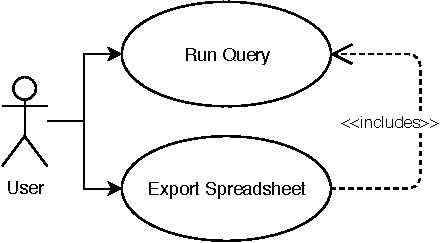
\includegraphics[width=.5\textwidth]{images/diagramas/userusecase}
  \caption{User use case}\label{fig:userusecase}
\end{figure}

\begin{figure}
  \centering
  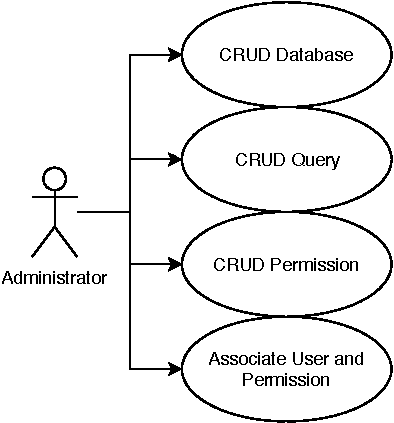
\includegraphics[width=.5\textwidth]{images/diagramas/adminusecase}
  \caption{Administrator use cases}\label{fig:adminusecases}
\end{figure}

According the intents of the stakeholders, this system should follow an architecture similar to that employed in their other projects, culminating to what is shown in Figure~\ref{fig:overview}, with an web front-end that is accessed by both actors to realize their use cases, a back-end service that provides business-specific functionalities and a database system to persist the system's own artifacts.

\begin{figure}
  \centering
  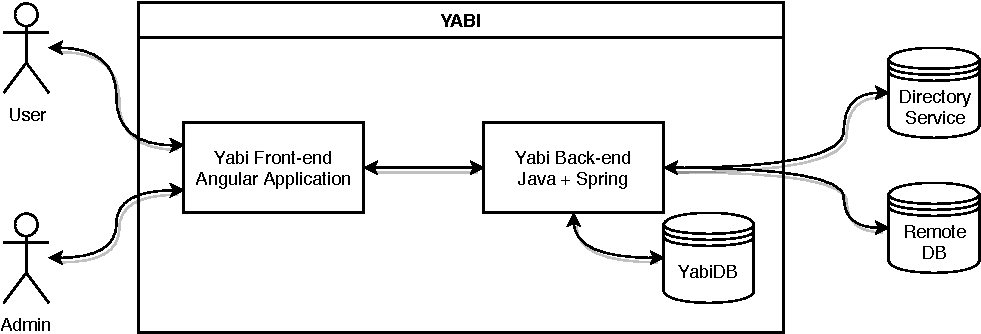
\includegraphics[width=\textwidth]{images/diagramas/overview.pdf}
  \caption{Yabi Overview}\label{fig:overview}
\end{figure}


\section{Conceptual Model}\label{tities}
When implementing the entities that were previously evaluated, it was found that some of the proposed names were reserved to \gls{RDBMS} and synonyms had to be used in the back-end, therefore Query became \texttt{SqlQuery}, User became \texttt{YabiUser} and Database became \texttt{Directory}. Permission is a separate case as it is not reserved by the \gls{RDBMS} and was instead named \texttt{PermissionTree} to express its tree-like behavior.

More concretely, the entities relate to themselves as shown in Figure~\ref{fig:er}. In sum, a Query is associated to a single Database and a single Permission, User on the other hand may have many Permissions and Permission has a relation to its parent.

\begin{figure}
  \centering
  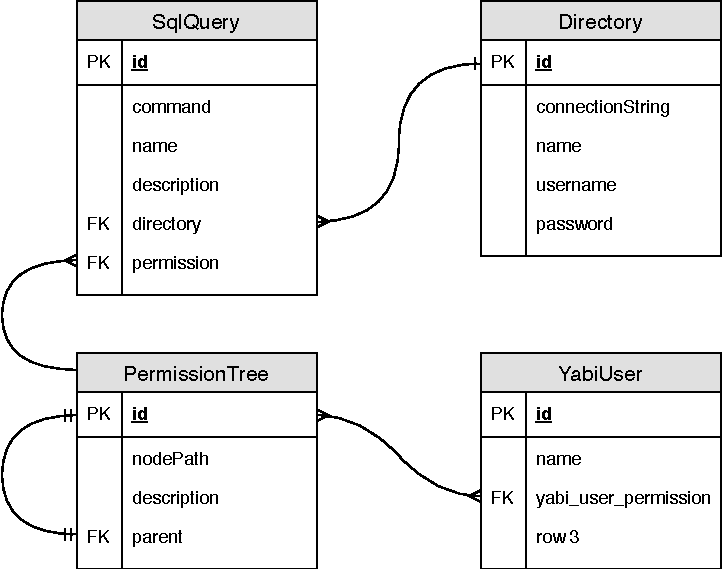
\includegraphics[width=.65\textwidth]{images/diagramas/er}
  \caption{Conceptual Model}\label{fig:er}
\end{figure}

\subsection{Project Details}\label{p:details}
Due to how the entities and their relations were designed, it is important to note some peculiarities and restrictions that came with it.

To begin with, Queries are associated to a single Permission and this led the listing of an User's Queries to be a unique list. An Administrator can manage all parts that are within this system's domain and thus, he cannot change the username as it is bound to the Directory Service. Every permission has a reference to its parent and the root Permission has a reference to itself. There are only two roles that any given user may be assigned to, either Administrator or User.

\section{Chapter Conclusion}

This chapter expressed the scope of the proposed application, how it was logically modeled and the requirements it was expected to meet.

In order to reduce the amount of interruptions received by the \gls{IT} department during student registration periods, this application seeks to give access to the information stored in \gls{IPB}'s databases in an organized manner. In sum, two actors were defined, the User whose main use cases consists of executing a Query and possibly downloading the results as a spreadsheet file and the Administrator, that associates one User with one or more Permissions.

The next chapter will be presenting how the entities and functionalities evaluated here were implemented into a functional application.